% !TEX encoding = UTF-8 Unicode


%%%%%%%%%%%%%%%%%%%%%%%%%%%%%%%%%%%%%%%%%%%%%%%%%%%%%%%
%%%%%%%%%%%%%%%%%%%%%%%%%%%%%%%%%%%% WPROWADZENIE
%%%%%%%%%%%%%%%%%%%%%%%%%%%%%%%%%%%%%%%%%%%%%%%%%%%%%%%
\chapter*{Wprowadzenie}
\label{chapter:wstep}
\thispagestyle{empty}


\rdm{
W rozdziale należy:
\begin{itemize}
\item zdefiniować dziedzinę wiedzy, do której nawiązuje tematyka pracy,
\item zdefiniować pojęcia występujące lub związane z tematem pracy, które definiują charakter pracy,
\item napisać motywację powstania pracy, tzn. wyjaśnić dlaczego autor uważa, że tematyka pracy jest istotna, opis motywacji powinien mieć ogólny charakter i być zrozumiały dla czytelnika nie będącego specjalistą w dziedzinie pracy, powinien odwoływać się do powszechnie spotykanych problemów i potrzeb,
\item sformułować cel/cele pracy,
\item opisać jakimi środkami informatycznymi zrealizowany zostanie cel pracy, jakie oprogramowanie zostanie zaimplementowane, jakie badania przeprowadzone, itp.,
\item przedstawić tezę pracy najlepiej używając sformułowania "jeżeli ... to ...",
\item opisać co znajduje się w kolejnych rozdziałach pracy: "W Rozdz.~\ref{chapter:przeglad} opisane zostały dotychczasowe pracy związane z ...",
\end{itemize}
}

\textcolor{red}{Tego rozdziału nie należy dzielić na mniejsze podrozdziały. Każdy z podpunktów powinien stanowić jeden akapit.}
 
 
 
%%%%%%%%%%%%%%%%%%%%%%%%%%%%%%%%%%%%%%%%%%%%%%%%%%%%%%%
%%%%%%%%%%%%%%%%%%%%%%%%%%%%%%%%%%%% PRZEGLĄD
%%%%%%%%%%%%%%%%%%%%%%%%%%%%%%%%%%%%%%%%%%%%%%%%%%%%%%% 
\chapter{\rdm{Przegląd istniejących rozwiązań w dziedzinie związanej z tematem pracy}}
\label{chapter:przeglad}
\thispagestyle{empty}

\rdm{Krótki opis tego co będzie omawiane w rozdziale.}

%%%%%%%%%%%% 
\section{\rdm{Wprowadzenie do tematyki pracy}}

\rdm{Opis zagadnień stanowiących podstawową wiedzę z tematyki poruszanej w pracy. Należy skoncentrować się na elementach, których poprawne zrozumienie jest najbardziej istotne z punktu widzenia zrozumienia treści pracy. Opisy pozostałych problemów powinno się potraktować pobieżnie odsyłając czytelnika do literatury.}

%%%%%%%%%%%% 
\section{\rdm{Klasyfikacja metod literaturowych}}

\rdm{Schemat przedstawiający ogólny obraz znanych metod wykorzystywanych do rozwiązywania problemów, którymi dyplomant zajmuje się w pracy. Krótki opis schematu klasyfikujący poszczególne metody.}

\begin{figure}[h!]
  \centering
  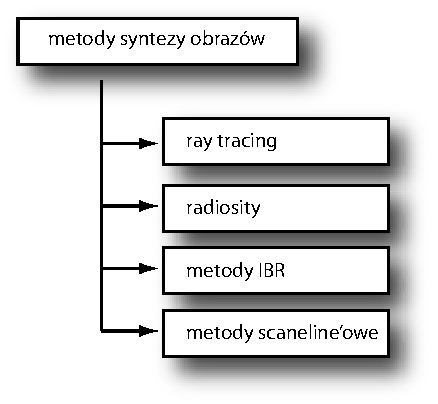
\includegraphics[width=0.5\linewidth]{rys/klasyfikacja}
  \caption{Klasyfikacja metod syntezy obrazów (źródło~\cite{Weis:1995}).}
  \label{fig:schemat}
\end{figure}


\subsection{\rdm{Opis metody literaturowej 1}}

\rdm{Skrótowy opis wybranej metody uwzględniający istotę jej działania oraz odesłanie do literatury, w której metoda jest omawiana w sposób szczegółowy. Porównanie opisywanej metody do rozwiązania proponowanego w pracy, krytyczna ocena metody.}


\subsection{\rdm{Cytowania}}

\rdm{Odsyłacze do pozycji literaturowej powinny wykorzystywać narzędzie \emph{bibtex} i mieć formę:~\cite[Rozdz.3.4]{Gamo:1995} lub~\cite{Weis:1995,Mantiuk13_GDOT,Tomaszewska07}. Treść stron internetowych może być również pozycją bibliograficzną. Proszę ją podawać w formie:~\cite{url_link} (trzeba zwrócić uwagę na zamieszczenie tytułu strony i w miarę możliwości autora treści strony). }


\subsection{\rdm{Jak zamieszczać rysunki?}}

\begin{itemize}
\item \rdm{W tekście pracy musi znajdować się odwołanie do każdego rysunku zamieszczonego w pracy, np. "Na Rys.~\ref{fig:schemat} prezentowany jest schemat...".}
\item \rdm{Napisy na rysunku powinny być wykonane czcionką o wielkości zbliżonej do czcionki podpisu pod rysunkiem.}
\item \rdm{Trzeba prawidłowo rozmieszczać rysunki, tzn. np. unikać sytuacji, w której mały rysunek zajmuje całą stronę.}
\item \rdm{Rysunki schematów należy wykonywać w formacie wektorowym (np. EPS lub PDF).}
\item \rdm{W przypadku rysunków bitmapowych trzeba zadbać o dostateczną ich rozdzielczość (minimum to 150~DPI, tzn. np. dla bitmapy zajmującej całą szerokość strony będzie to około 900 pikseli).}
\end{itemize}


\subsection{\rdm{Jak formatować tekst?}}

\begin{itemize}
\item \rdm{Aby wyróżnić wyraz/frazę proszę stosować konstrukcję:  \emph{wyróżniona fraza}. Takie wyróżnienie stosuje się do ważnych nowych pojęć wprowadzanych po raz pierwszy w tekście pracy (np. nazwa algorytmu, technologii, itp.).}
\item \rdm{W przypadku używania niepopularnego określenia angielskiego terminu, warto po polskim tłumaczeniu podać wersję angielską w formie: obrazy o rozszerzonym zakresie dynamiki (ang. \emph{high dynamic range images}).}
\item \rdm{Na końcu tytułów rozdziałów/podrozdziałów NIE stawiamy kropek.}
\item \rdm{Na końcu podpisów pod rysunkami/tabelami stawiamy kropki.}
\end{itemize}

\subsection{\rdm{Przykład zamieszczania wzorów}}

\rdm{W równaniu:}

\begin{equation}
\label{equation:1}
    x = R_{0} + s \cdot R_{time},
\end{equation}

\rdm{gdzie parametr $s$:}

\begin{displaymath}
\label{equation:2}
    s = c \cdot (t_{0} - time)
\end{displaymath}

\rdm{zdefiniowano zależność opisującą zmianę prędkości obiektu. Parametr $t_{0}$ wyraża czas na początku pomiaru, $time$ bieżący czas, $R_{0}$ prędkość w chwili $t_{0}$, natomiast $R_{time}$ prędkość w chwili $time$. $c$ jest stałą wyznaczoną w eksperymencie.}


\rdm{Proszę zwrócić uwagę na przecinki i kropki na końcu wzorów. Wzór jest częścią zdania, musi więc podlegać regułom budowania zdań. W tekście pracy do każdego wzoru oznaczonego numerem musi znajdować się odwołanie: (patrz równanie~\ref{equation:1}). Każdy element wzoru powinien zostać jednoznacznie zdefiniowany.}


\subsection{\rdm{Podsumowania}}

\rdm{Podsumowanie skuteczności/nieskuteczności metod literaturowych i wskazanie dlaczego w pracy proponowana jest nowa metoda. Pod jakimi obiektywnymi względami nowa metoda jest lepsza od tych opisanych w literaturze.}




%%%%%%%%%%%%%%%%%%%%%%%%%%%%%%%%%%%%%%%%%%%%%%%%%%%%%%%
%%%%%%%%%%%%%%%%%%%%%%%%%%%%%%%%%%%% METODA
%%%%%%%%%%%%%%%%%%%%%%%%%%%%%%%%%%%%%%%%%%%%%%%%%%%%%%% 
\chapter{\rdm{Opis metody rozwiązania problemu prezentowanego w pracy}}
\label{chapter:metoda}
\thispagestyle{empty}

\rdm{Krótki opis co znajdzie się w rozdziale.}\\

%%%%%%%%%%%% 
\section{\rdm{Ogólny opis metody}}

\rdm{Opis metody, za pomocą której rozwiązano problem w pracy. Powinna to być prezentacja metody nie nawiązująca do jej implementacji. Istotne jest wyjaśnienie podstaw matematycznych i/lub fizycznych działania metody. Przedstawienie algorytmu jako całości, zdefiniowanie modułów i powiązań między modułami. Zdefiniowanie interfejsów (wejścia i wyjścia). W kolejnych podpunktach należy ze szczegółami omówić konkretne rozwiązania stosowane w metodzie. }

\rdm{W tym rozdziale rekomendowane jest zamieszczenie ogólnego schematu działania opisywanej techniki/metody.}

\rdm{W przypadku prac inżynierskich Rozdz.~\ref{chapter:metoda} może zostać połączony z Rozdz.~\ref{chapter:implementacja}.}

%%%%%%%%%%%% 
\subsection{\rdm{Opis zagadnienia szczegółowego 1}} 

\rdm{Charakterystyka zagadnienia.}\\

%%%%%%%%%%%% 
\subsection{\rdm{Opis zagadnienia szczegółowego 2}}

\rdm{Charakterystyka zagadnienia.}\\


%%%%%%%%%%%%%%%%%%%%%%%%%%%%%%%%%%%%%%%%%%%%%%%%%%%%%%%
%%%%%%%%%%%%%%%%%%%%%%%%%%%%%%%%%%%% IMPLEMENTACJA
%%%%%%%%%%%%%%%%%%%%%%%%%%%%%%%%%%%%%%%%%%%%%%%%%%%%%%% 
\chapter{\rdm{Opis implementacji metody}}
\label{chapter:implementacja}
\thispagestyle{empty}

\rdm{Krótki opis tego co znajdzie się w rozdziale.}

%%%%%%%%%%%% 
\section{\rdm{Schemat implementacji}}

\rdm{Ogólny schemat implementacji pozwalający czytelnikowi na łatwe zrozumienie struktury oprogramowania, powiązania pomiędzy elementami systemu, itp.}

\subsection*{Opis środowiska}

\rdm{Charakterystyka środowiska, w którym zaimplementowano metodę oraz  środowiska, w którym ją testowano. Dane techniczne użytego sprzętu i oprogramowania (dokładna specyfikacja sprzętu, numery wersji oprogramowania, które decyduje o wydajności implementacji). Opis konfiguracji sprzętowej oraz konfiguracji użytego oprogramowania (schematy).}

\subsection*{Format danych wejściowych oraz wyjściowych}

\rdm{Definicja formatu danych wejściowych oraz opis generowanego formatu wyjściowego.} 

%%%%%%%%%%%% 
\section{\rdm{Opis implementacji metody}}

\rdm{Opisy charakterystycznych elementów implementacji:}

\begin{itemize}
\item{\rdm{można zamieszać fragmenty kodów źródłowych bądź pseudokody fragmentów programu.}}

\rdm{Przykład sposobu zamieszczenia kodu źródłowego:}
\small
\begin{verbatim}

for(i = 0; i < 10; i++){         // licznik od 1 do 10
    i = i + 1;                // zwiększenie licznika
    printf("Licznik:%d\n", i);	    // wizualizacja wyniku
}
\end{verbatim}

\rdm{Każda linia kodu musi być opisana. Proszę zwrócić uwagę na poprawne formatowanie kodu.}

\normalsize

\item{\rdm{opis działania programu (pomocne jest zamieszczanie rysunków prezentujących poszczególne fazy działania programu),}}
\item{\rdm{opis głównych opcji/trybów dostępnych w implementacji oprogramowania (szczegółową charakterystykę opcji należy zamieścić w dodatku),}}
\item{\rdm{opis problemów napotkanych w czasie implementacji metody.}}

\end{itemize}



%%%%%%%%%%%%%%%%%%%%%%%%%%%%%%%%%%%%%%%%%%%%%%%%%%%%%%%
%%%%%%%%%%%%%%%%%%%%%%%%%%%%%%%%%%%% REZULTATY
%%%%%%%%%%%%%%%%%%%%%%%%%%%%%%%%%%%%%%%%%%%%%%%%%%%%%%% 
\chapter{Rezultaty i wnioski}
\label{chapter:rezultaty}
\thispagestyle{empty}

\rdm{Krótki opis tego co znajdzie się w rozdziale.}

%%%%%%%%%%%% 
\section{Opis procedury testowej}

\rdm{W podrozdziale tym należy opisać:}
\begin{itemize}
\item{\rdm{jaki jest cel przeprowadzenia testów (co testy mają wykazać),}}
\item{\rdm{co będzie metryką pozwalającą na ocenę jakości uzyskanych rezultatów (polecane jest stosowanie metryk porównawczych, tzn. np. porównanie jakości obrazu do obrazu wzorcowego),}}
\item{\rdm{jakie testy zostaną przeprowadzone,} }
\item{\rdm{należy wyspecyfikować procedurę testową w stopniu umożliwiającym czytelnikowi jej powtórzenie,}}
\item{\rdm{jakie dane wejściowe zostaną użyte w testach (np. jakie obrazy testowe).}}
\end{itemize}

%%%%%%%%%%%% 
\section{Prezentacja rezultatów}

\begin{table}
\begin{center}
\caption[Tabela ]{Prezentacja formatowania tabeli}
\begin{tabular}{|l|c|r|}
\hline
{\bf kolumna 1} & {\bf kolumna 2} & {\bf kolumna 3} \\
\hline
ent5 & ent6 & ent7  \\
\hline
ent10 & ent11 & ent12 \\
\hline
ent15 & ent16 & ent17 \\
\hline
ent20 & ent21 & ent22 \\
\hline
ent25 & ent26 & ent27 \\
\hline
ent30 & ent31 & ent32 \\
\hline
\end{tabular}
\label{table:przyklad}
\end{center}
\end{table}
\rdm{
Przykład formatowania tabeli: \ref{table:przyklad}.
}

\rdm{
\begin{itemize}
\item{Prezentacja rezultatów - tabele z wynikami, wykresy.}
\item{Komentarz do uzyskanych wyników (w szczególności trzeba opisać wyniki najlepsze i najgorsze).}
\item{Wyjaśnienie przyczyny pojawienia się błędnych rezultatów.}
\item{Porównanie rezultatów z danymi wzorcowymi.}
\end{itemize}}

%%%%%%%%%%%% 
\section{Wnioski}

\rdm{Ogólne wnioski dotyczące uzyskanych rezultatów. Dyskusja jak wypadają uzyskane wyniki na tle danych wzorcowych.}


%%%%%%%%%%%%%%%%%%%%%%%%%%%%%%%%%%%%%%%%%%%%%%%%%%%%%%%
%%%%%%%%%%%%%%%%%%%%%%%%%%%%%%%%%%%% PODSUMOWANIE
%%%%%%%%%%%%%%%%%%%%%%%%%%%%%%%%%%%%%%%%%%%%%%%%%%%%%%% 
\chapter*{Podsumowanie oraz dalsze prace}
\label{chapter:wstep}
\thispagestyle{empty}

\rdm{
W rozdziale tym należy:
\begin{itemize}
\item {podsumować co zostało wykonane w pracy (4-5 zdań),}
\item{stwierdzić, że uzyskane wyniki potwierdzają zrealizowanie celu pracy,}
\item {wymienić wszystkie elementy, które zostały wykonane w pracy w kolejności od najważniejszych (np. opracowanie analitycznej metody rozwiązania problemu X) do mniej istotnych (np. sklasyfikowanie metod literaturowych).}
\end{itemize}
}

\subsection*{Dalsze pracy} %%%%%%%%%%%% 

\rdm{Obszernie opisać w jakim kierunku można dalej rozwijać projekt. Wskazać co nie zostało zrealizowane lub nie zostało dokończone, jednocześnie wskazując na obiektywne przyczyny takiej sytuacji.}





